%\includegraphics[width=0.8\linewidth]{3.jpg}
\section{Architecture}

As described before, the three main data sources that the algorithm uses are FMS bus, accelerometer sensor and GPS sensor. Since the overall available data is much larger than the data required by the algorithm, the corresponding API is provided for each data source. In addition to the encapsulation role these interfaces have, they can be extended for the future use as well, in the case of additional modifications or improvements. Moreover, a layer is added above the accelerometer and GPS API in order to maintain the acquired data and provide further actions.
\begin{figure}[!htb]
	\makebox[\textwidth]{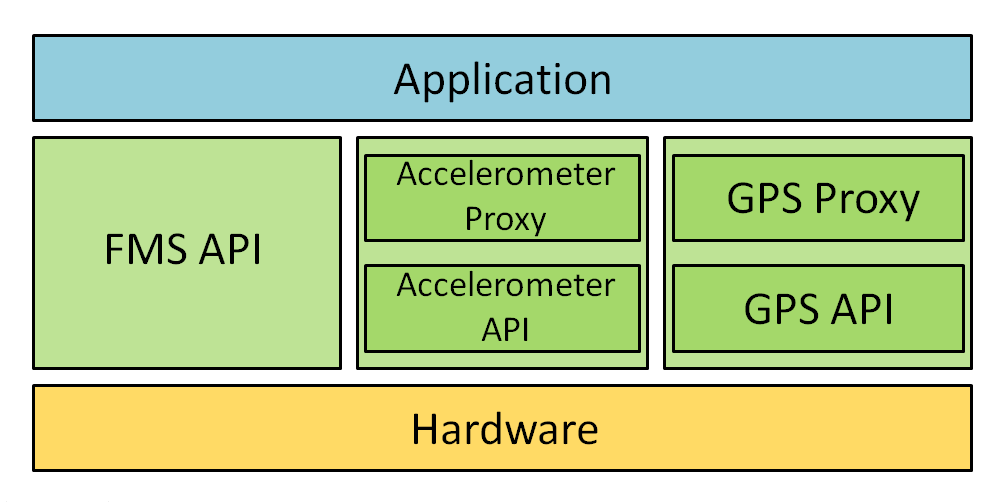
\includegraphics[width=\textwidth]{architecture}}\caption{Architecture}
    \label{fig::architecture}
\end{figure}
\\
As it is shown in the Figure \ref{fig::architecture}, the architecture is layer based. The higher layers abstract from lower layers, while the lower layers do not know about higher layers. Nevertheless, not all the communication links are permitted. Allowed ones are only the module based communication links into the directly lower level. That being said, neither the horizontal communication nor bypassing the layers is permitted. Currently, the only present communication is top-down by function calls, but the possible one could also be bottom-up by triggering some event. This structure improves the maintainability and scalability on the one hand, but in contrast, it could increase a communication load significantly with including more functions to the algorithm. 
\clearpage
